\begin{figure}[h]
    \centering
    \begin{subfigure}[b]{0.3\textwidth}
        \centering
        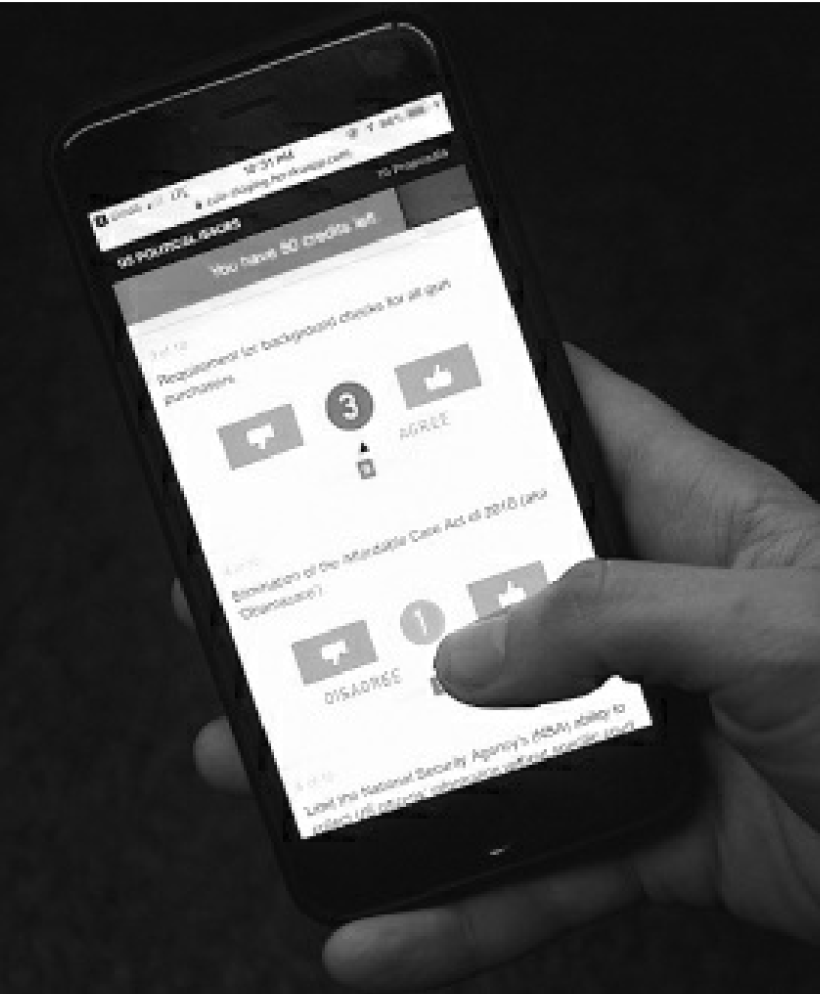
\includegraphics[width=\textwidth]{content/image/curr_interface/radical_market_wedesign.png}
        \caption{Software designed by WeDesign used in~\cite{quarfoot2017quadratic}. Image taken from~\cite{posner2018radical}.}
        \label{fig:wedesignInterface}
    \end{subfigure}
    \hfill
    \begin{subfigure}[b]{0.3\textwidth}
        \centering
        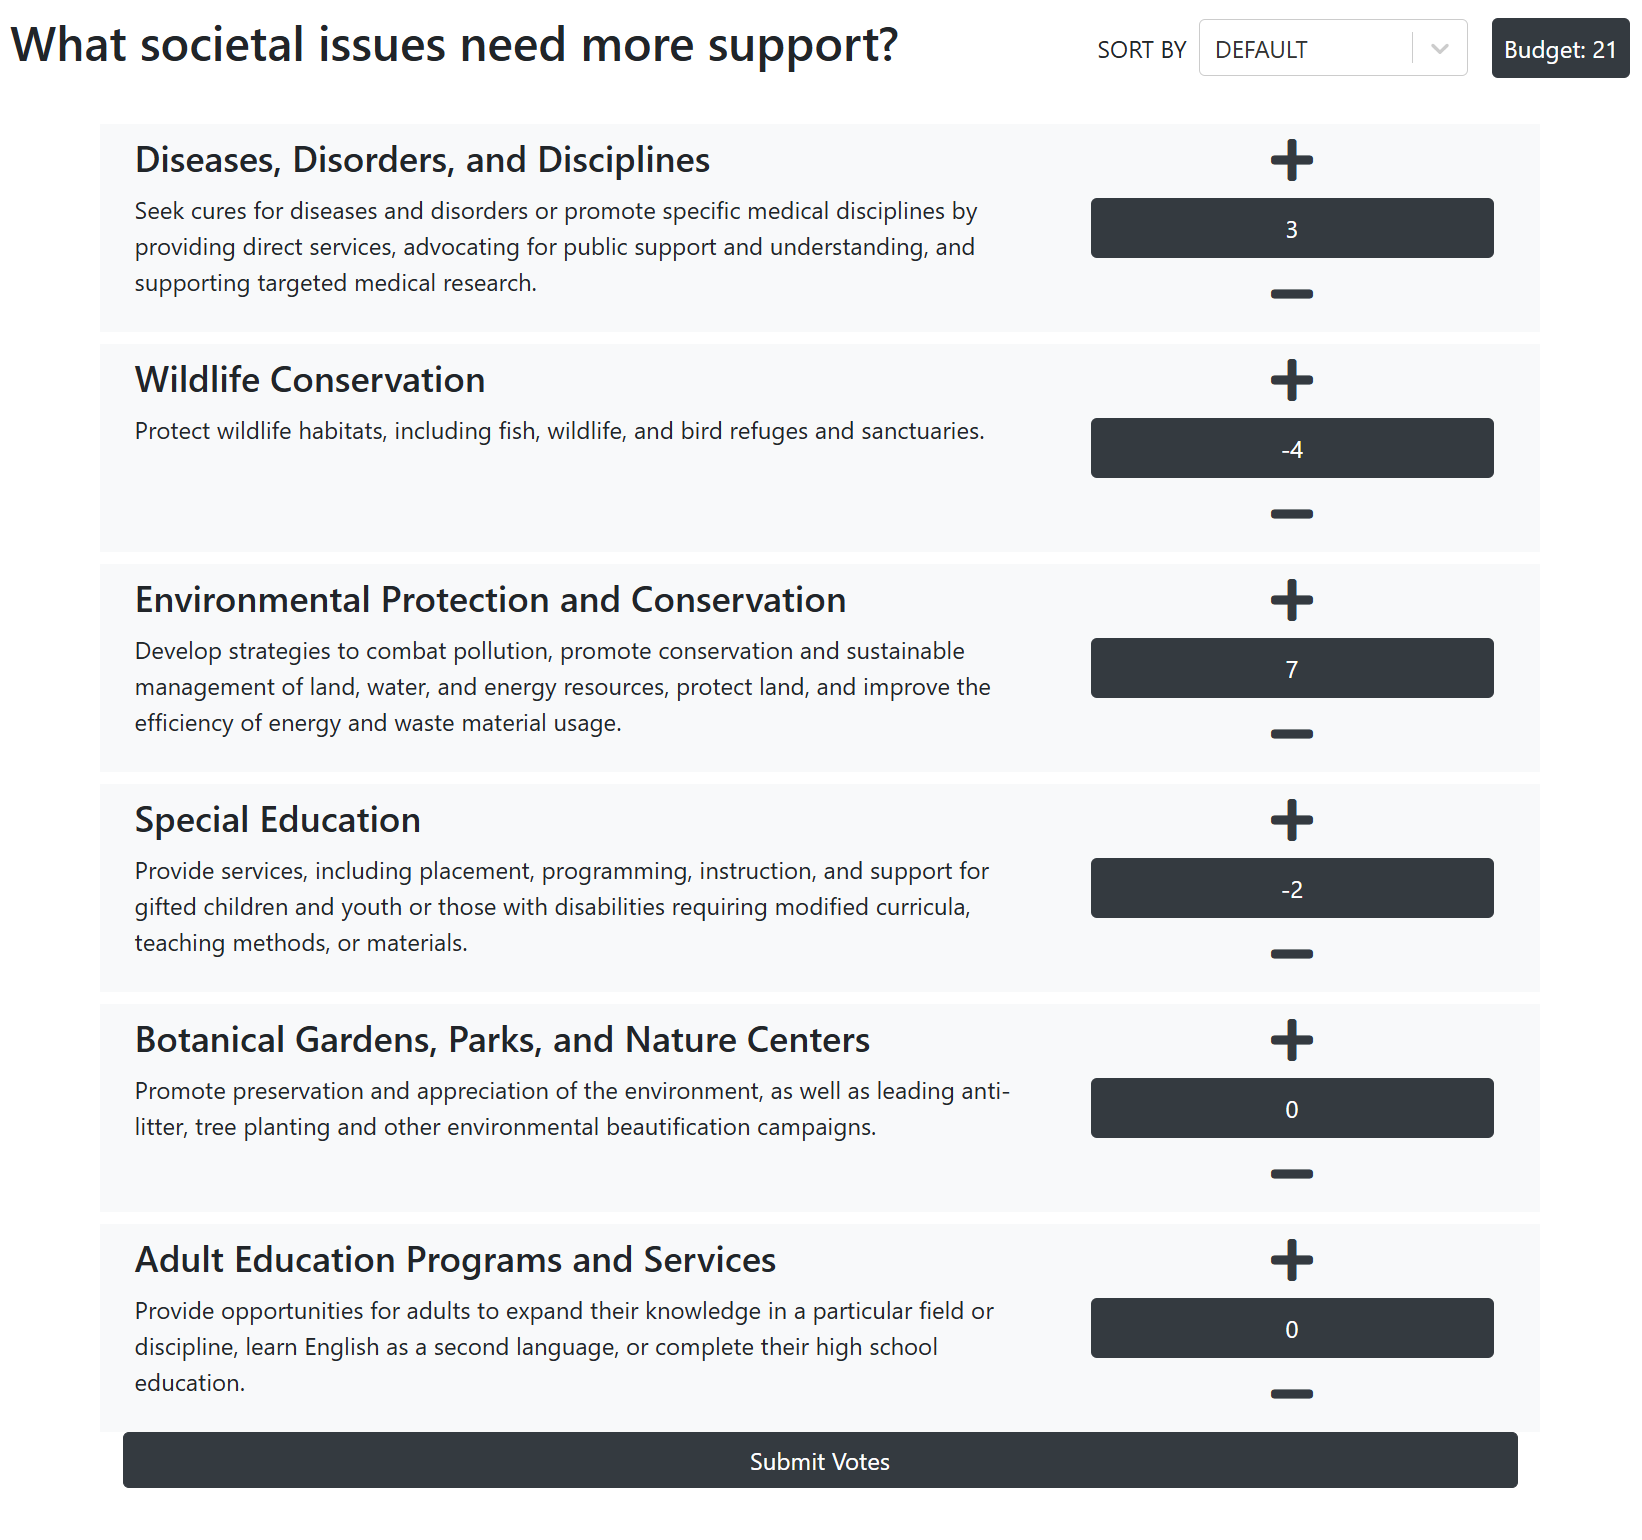
\includegraphics[width=\textwidth]{content/image/curr_interface/geek.sg_interface.png}
        \caption{An open-source QV interface~\cite{yehjxraymondYehjxraymondQvapp2024} with a publicly available service.}
        \label{fig:yehInterface}
    \end{subfigure}
    \hfill
    \begin{subfigure}[b]{0.3\textwidth}
        \centering
        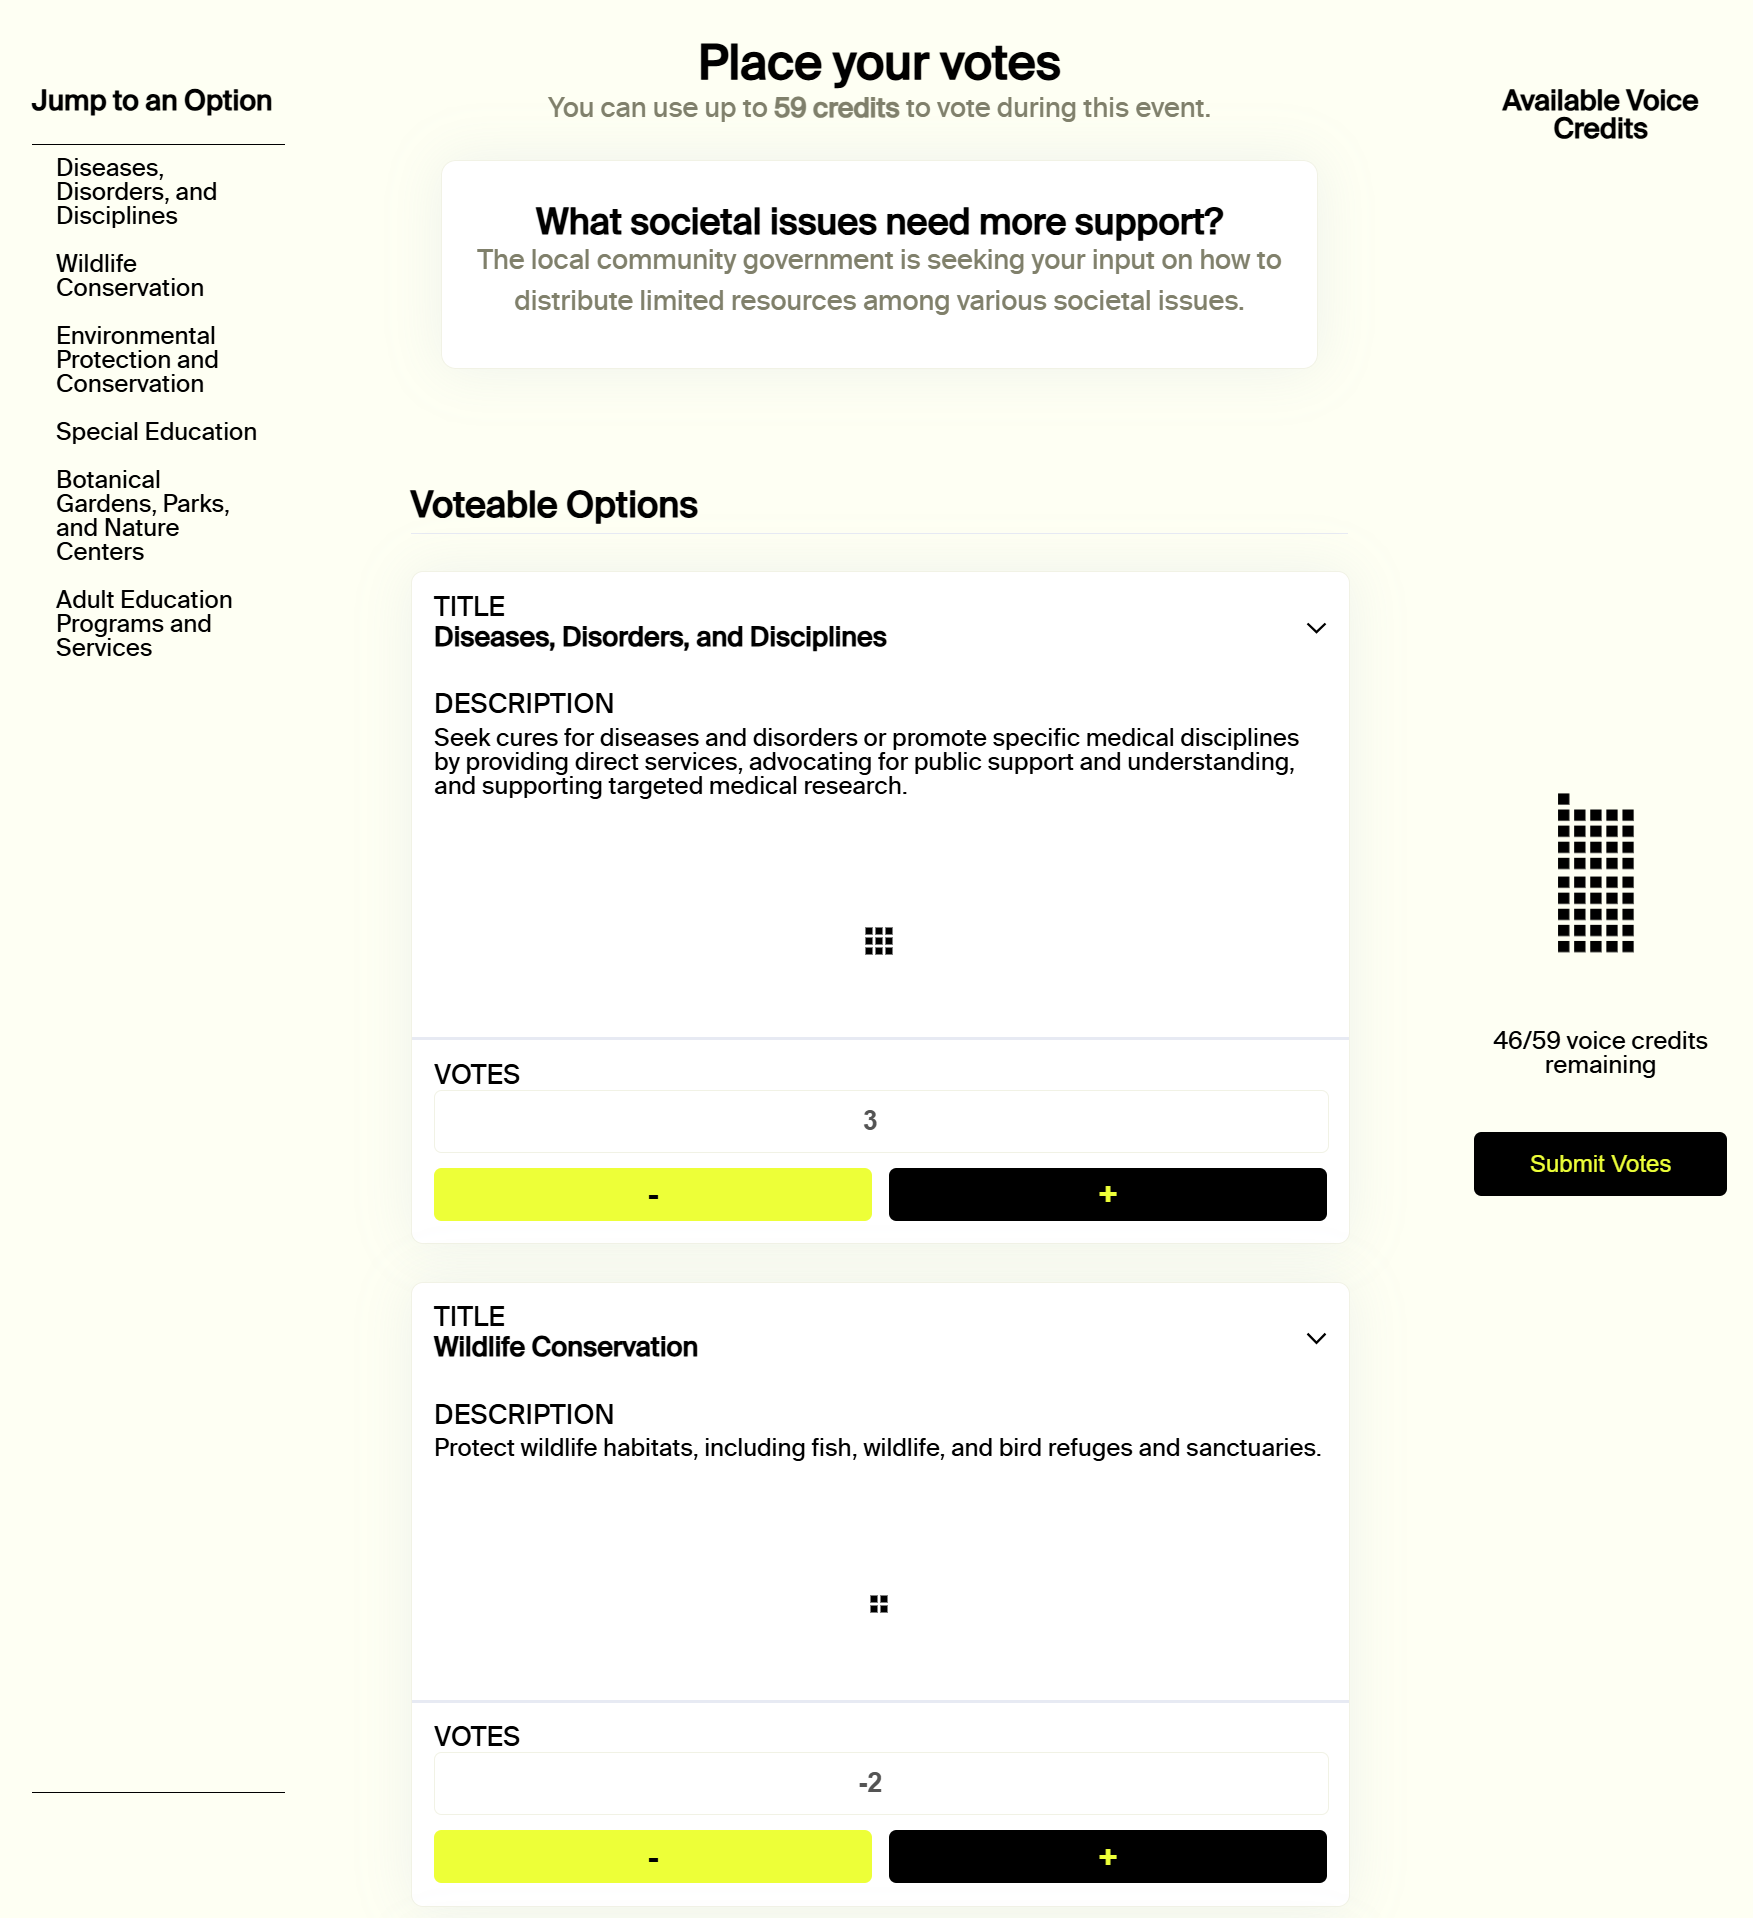
\includegraphics[width=\textwidth]{content/image/curr_interface/rxc_interface.png}
        \caption{An open-source QV interface~\cite{RadicalxChangeQuadraticvoting2024} forked from GitCoin~\cite{ReadWhitepaperGitcoin} used by the RadicalxChange community~\cite{RxC}.}
        \label{fig:rxcvotingInterface}
    \end{subfigure}
    \vskip\baselineskip
    \begin{subfigure}[b]{0.3\textwidth}
        \centering
        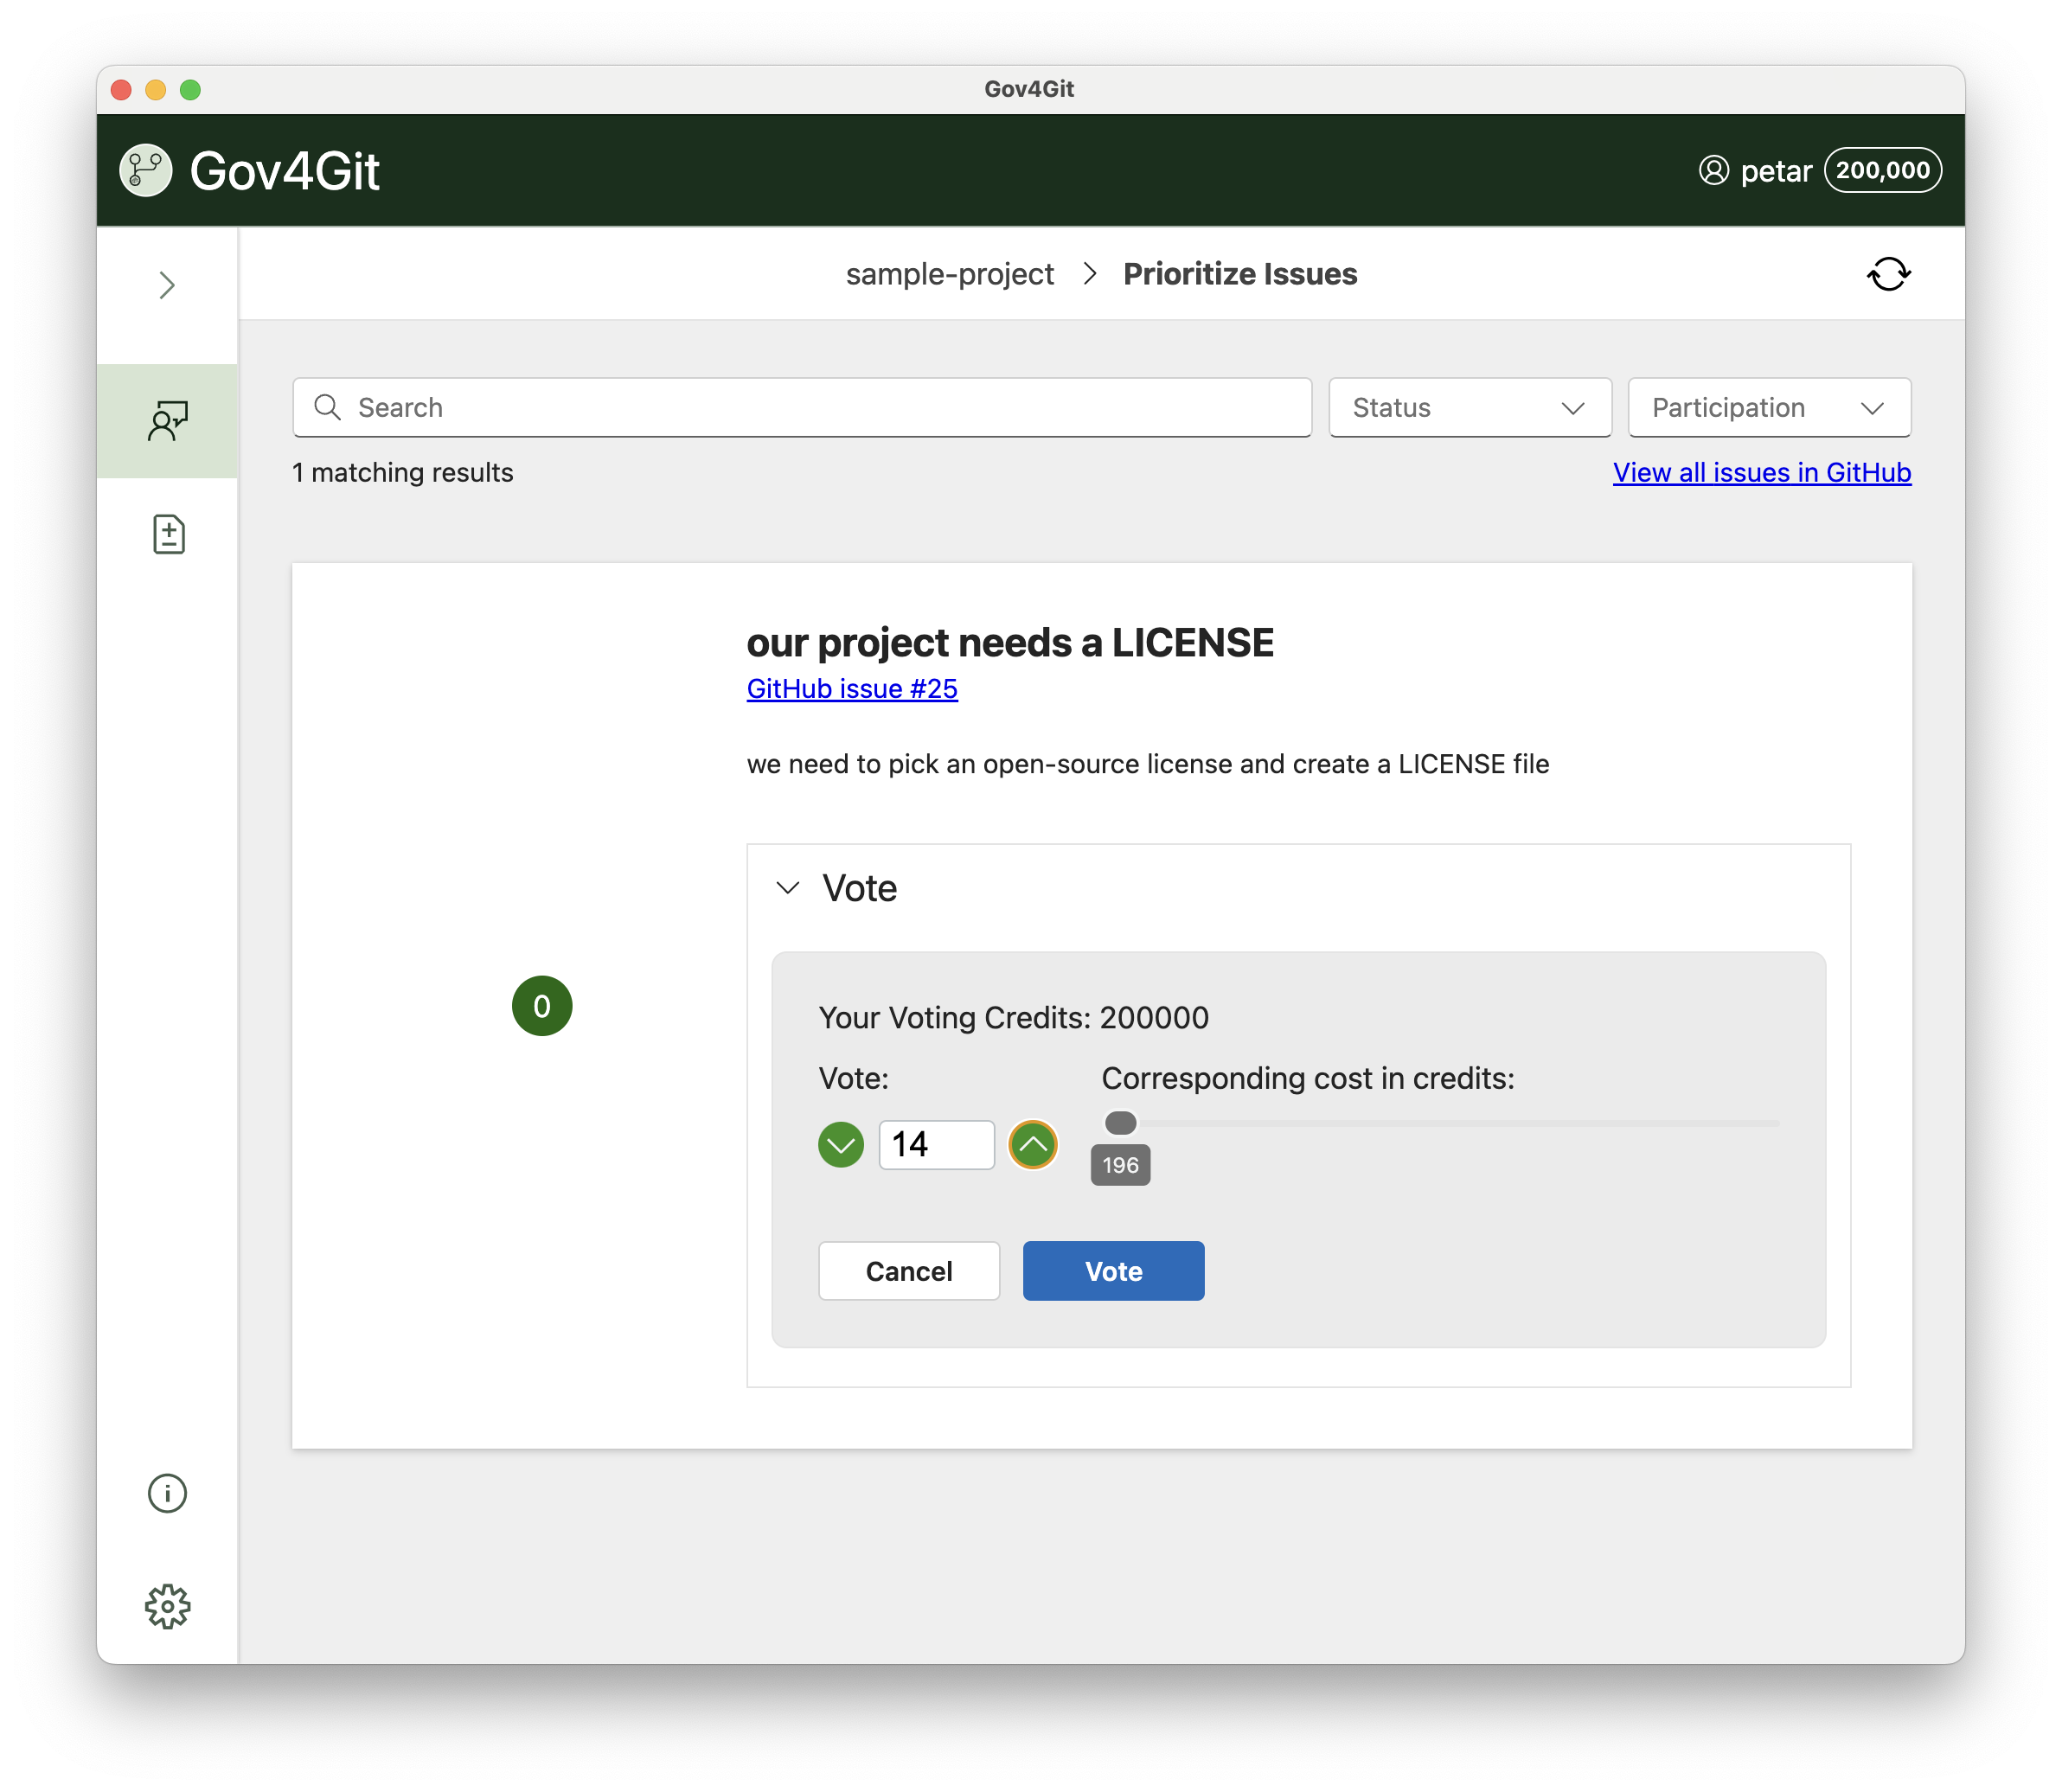
\includegraphics[width=\textwidth]{content/image/curr_interface/appvote.png}
        \caption{The interface designed for gov4git~\cite{Gov4gitDecentralizedPlatform2023}.}
        \label{fig:gov4gitInterface}
    \end{subfigure}
    \begin{subfigure}[b]{0.3\textwidth}
        \centering
        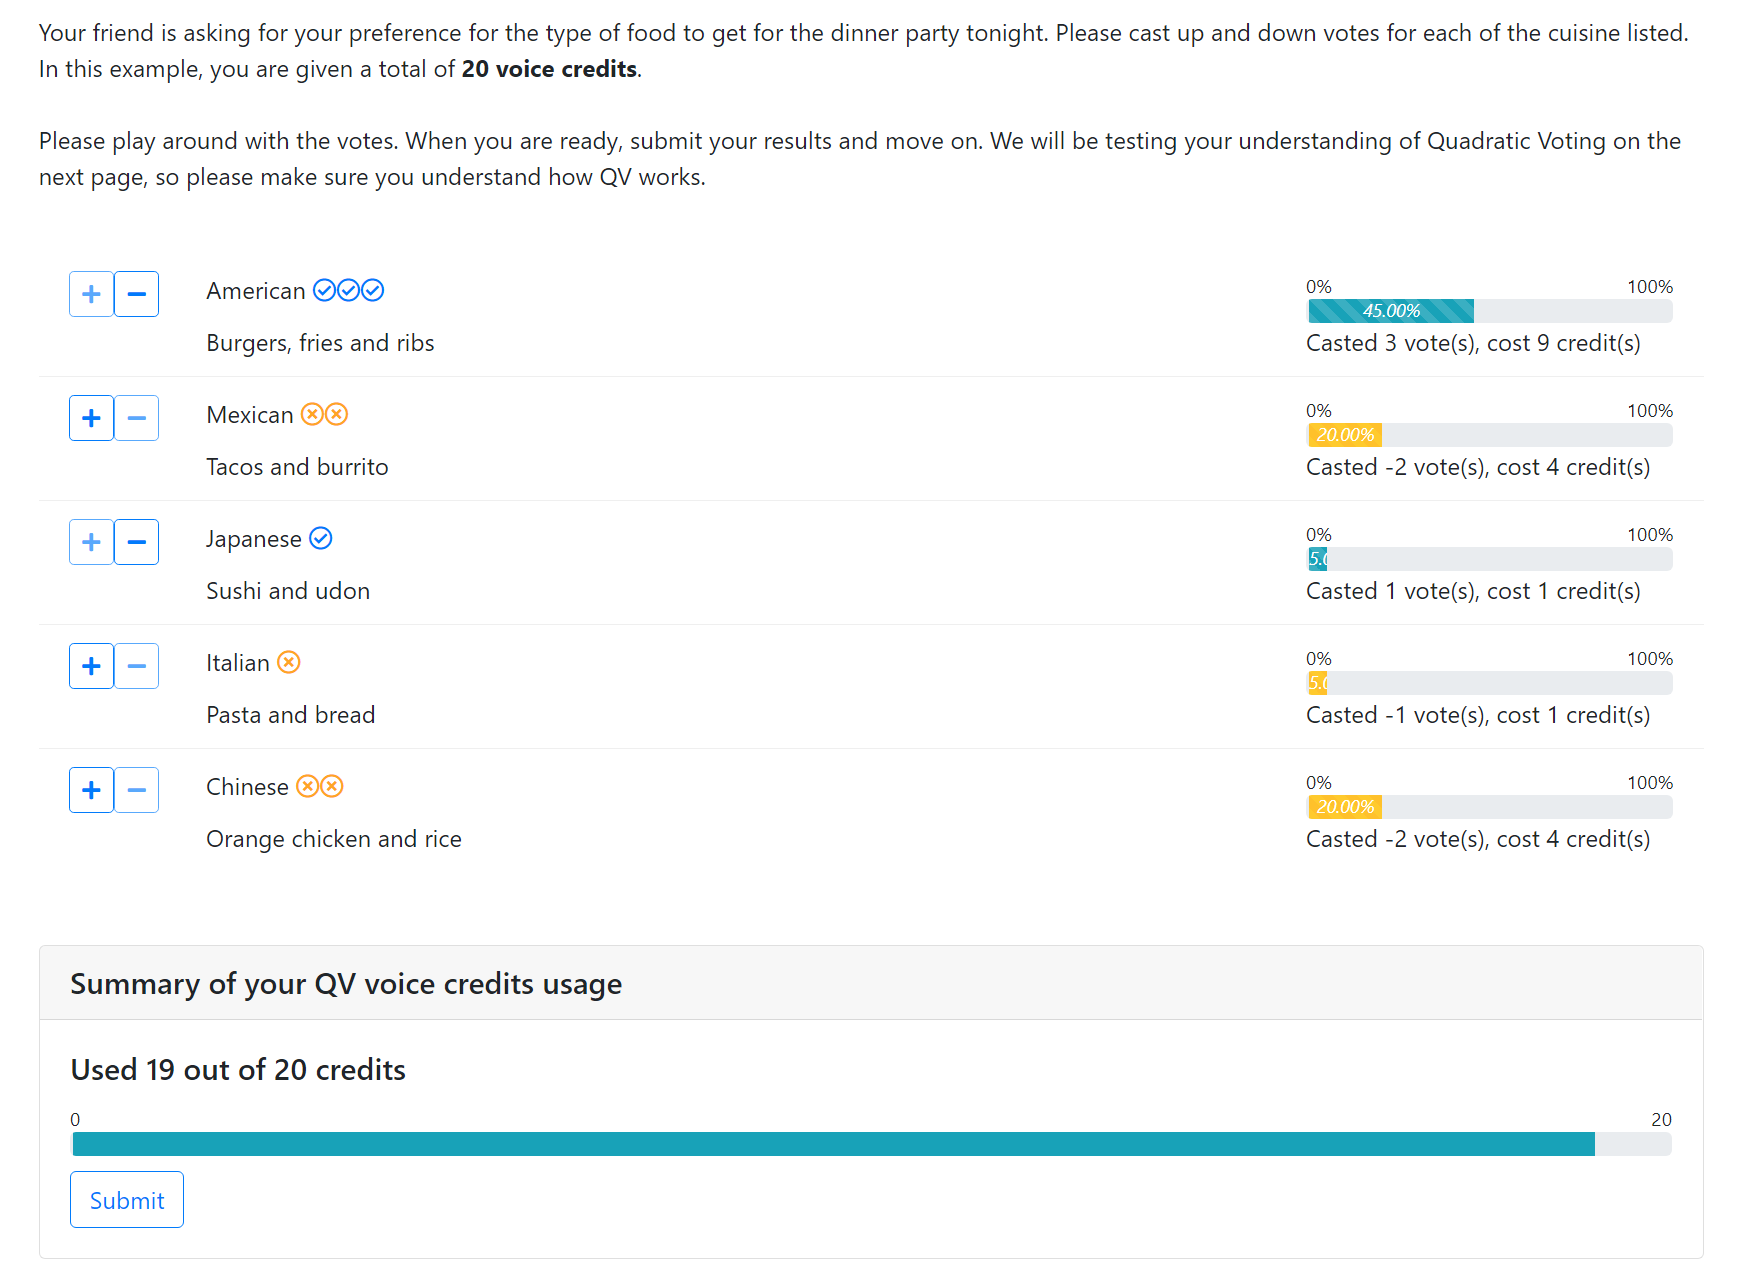
\includegraphics[width=\textwidth]{content/image/curr_interface/cheng_qv.png}
        \caption{The interface used in the research by~\textcite{chengCanShowWhat2021}.}
        \label{fig:chengInterface}
    \end{subfigure}
    \caption{Recent implementations of interfaces applying the quadratic mechanism.}
    \label{fig:qv_interface_external}
\end{figure}

\section{Interface Design}
\label{sec:interfaceDesign}
In this study, we developed an interactive interface for QS based on prior literature for the experiment condition. As there no standardlized QV interface, we constructed a text based QS interface that includes most of what existing interfaces offers and make it comparable with the interactive interface. In the following subsections, we describe these interface design decisions and supporting literature.

\begin{figure}[H]
    \centering
    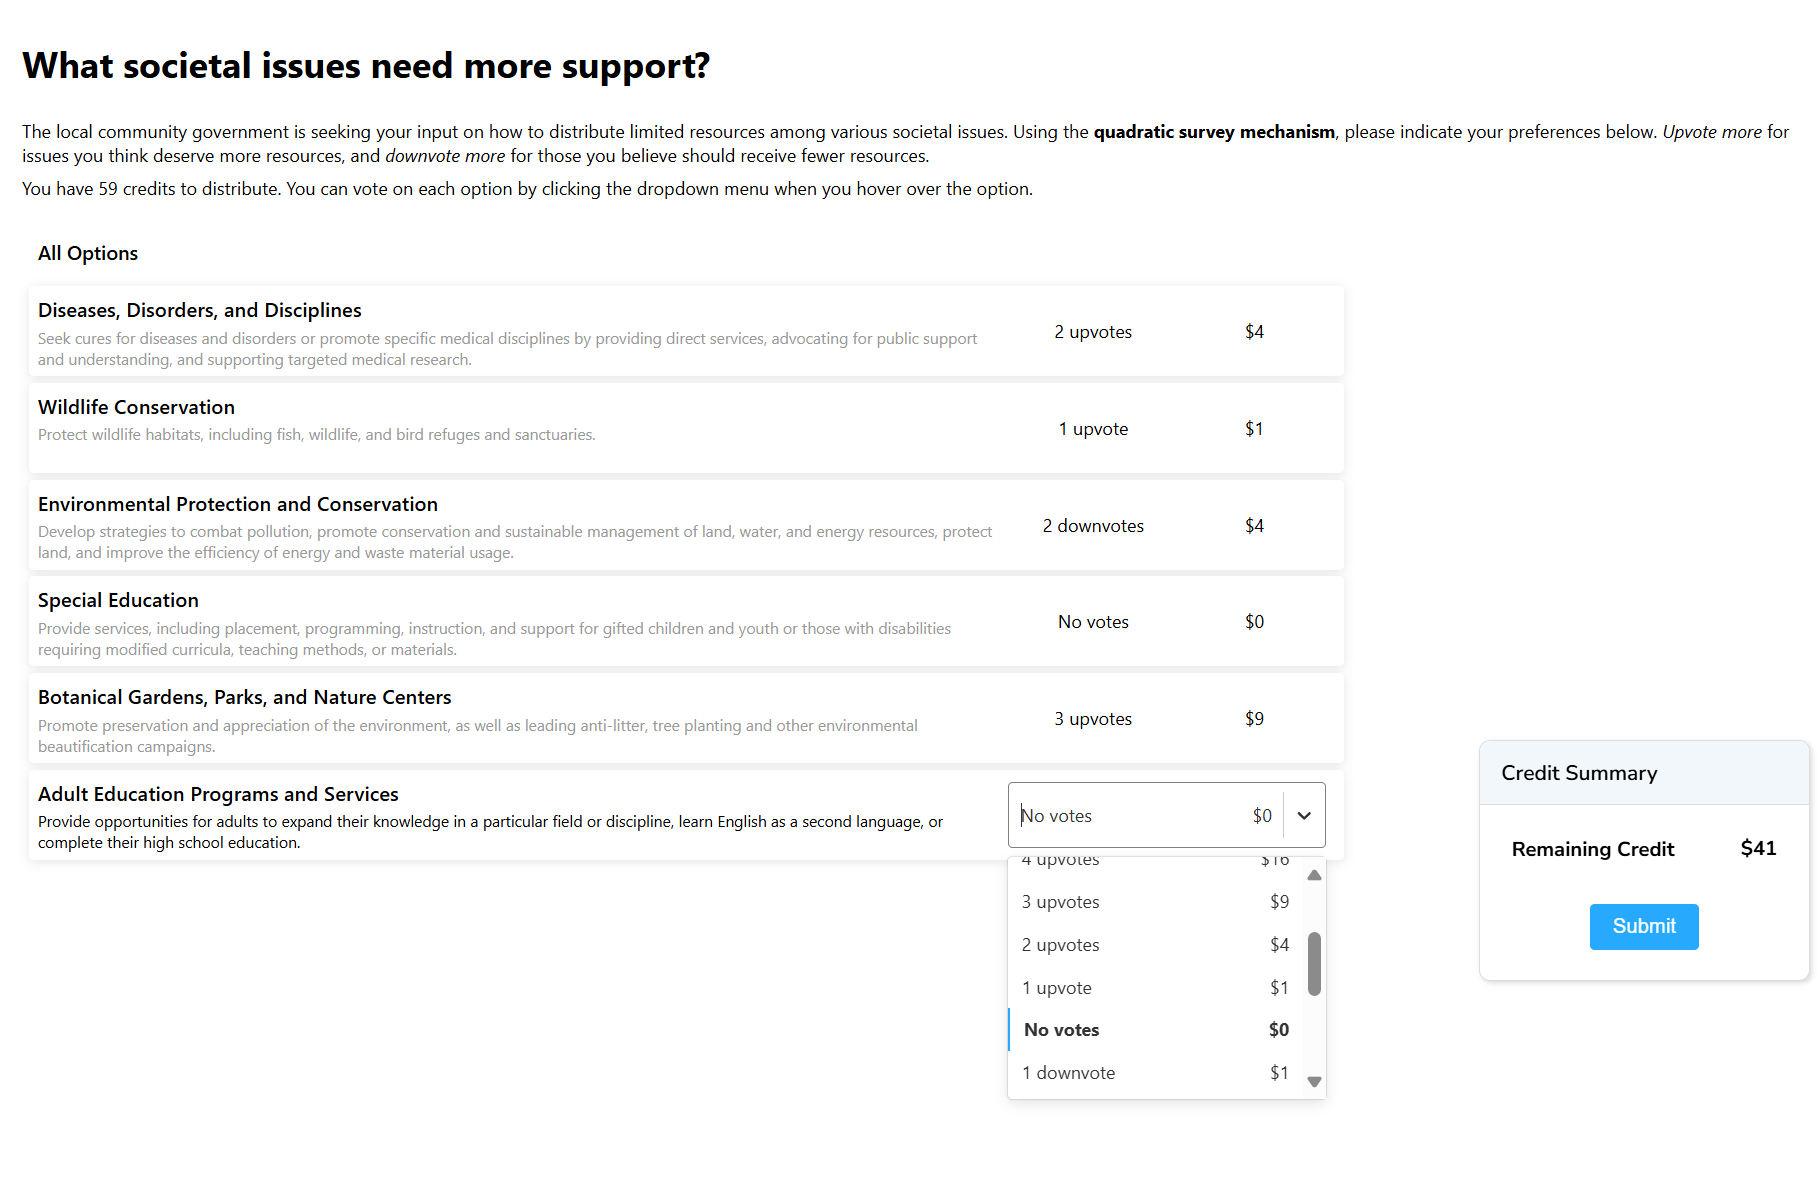
\includegraphics[width=0.6\textwidth]{content/image/text_interface.png}
    \caption{The text-based interface}
    \label{fig:textInterface}
\end{figure}

\subsection{Text-based Interface (Text Condition)}
First, we surveyed the current implementation of QV interfaces to understand the development of such tools. We present a selection in Figure~\ref{fig:qv_interface_external}. All five interfaces retain and present the following components:
\begin{itemize}
    \item Option list: A list of options contesting for votes.
    \item Vote Controls: Two buttons to increase and decrease votes associated with an option.
    \item Individual vote counts: Some representation of the number of votes associated with an option.
    \item Summary: A summary automatically calculates the cost of the total votes.
\end{itemize}

We constructed a text-based interface that included all five components but removed the use of emojis (i.e., thumbs up and thumbs down present in Figure~\ref{fig:wedesignInterface}), progress bars, and other visualizations in the summary section (i.e., progress bars in Figure~\ref{fig:wedesignInterface} and~\ref{fig:chengInterface} or blocks presented in Figure~\ref{fig:rxcvotingInterface}), and the visual cues for individual vote counts (i.e., the colored counts and icons present in Figure~\ref{fig:gov4gitInterface} and~\ref{fig:chengInterface}). Prior literature suggests that the use of emojis might influence the interpretations of surveys~\cite{herringGenderAgeInfluences2020} and decrease user satisfaction~\cite{toepoelSmileysStarsHearts2019}. We also removed all visualization elements such as blocks, progress bars, and percentage indicators, as prior literature shows that not all data visualization elements reduce cognitive demand~\cite{huangMeasuringEffectivenessGraph2009a}. Last, we decided to present all the options on the same screen. Prior research emphasizes the importance of placing all the options on the same digital ballot screen to avoid losing votes (missing citations). This echoes the proverb ``out of sight, out of mind,'' where individuals might be biased toward options that are shown to them and additional effort is required for individuals to retrieve specific information if options are hidden (citation needed).



These design decisions led to the interface shown in Figure~\ref{fig:textInterface}. The interface contains the question prompt at the top of the screen. The options are presented as a list of options below it. Survey respondents can update the votes, showing the cost and the number of votes, by selecting from a dropdown that provides all possible voting options and cost given the number of credits. A small summary box to the right of the interface shows the current total cost and the remaining credit for the respondent. To avoid ordering bias~\cite{ferberOrderBiasMail1952, couperWebSurveyDesign2001}, options are always randomly presented on the interface.

\subsection{Interactive Interface (Interactive Condition)}
The interactive interface, shown in Figure~\ref{fig:interactiveInterface}, builds additional interactive elements on top of the text interface to maintain consistency that allows comparison of the direct manipulation of the designed interactive elements. We designed two additional components: An additional organization step prior to voting and a drag-and-drop interface throughout the QS responding session informed through prior literature.

\paragraph{Organization Phase}

The design of the organization phase in this interactive interface began from understanding~\textcite{strackThinkingJudgingCommunicating1987}'s research on how survey respondents process and respond to attitude surveys. They propose that individuals, after comprehending a question, would either recall a previous judgment or construct a new one. This organization phase is designed to guide respondents through the process of forming opinions on individual options incrementally and methodically.

The organizing interface, as shown on the left-hand side of Figure~\ref{fig:interactiveInterface}, begins by presenting all survey options one at a time right under the system prompt. Survey respondents select a response among three ordinal categories -- lean positive, lean negative, or lean neutral. Once selected, the system will move that option to the respective category. Participants can skip the option if they do not want to indicate a preference. Options within the groups are draggable and rearrangeable to other groups should the participants want. In other words, we designed an interface to nudge survey respondents to review and group different options.

Three theoretical theories informed such design. First, to reduce cognitive load, showing participants one option at a time gated the amount of information presented to the survey respondent and thereby reduced the extraneous load~\cite{swellerCognitiveLoadTheory2011}. The three possible options, positive, neutral, and negative, aim to scaffold participants in constructing their own choice architecture~\cite{munscherReviewTaxonomyChoice2016, thalerNudgeImprovingDecisions2008a}, which strategically segments options into diverse and alternative choice presentations while avoiding the biases from defaults. The immediate feedback and the agency for participants to edit their `categorization' stem from basic HCI principles~\cite{norman2013design}. This design underwent paper prototypes and various iterations, which all maintained the combination of these theoretical bases aimed at reducing cognitive load and scaffolding the decision-making process. We describe these iterations and the design process in Appendix A.

\begin{figure}[h]
    \centering
    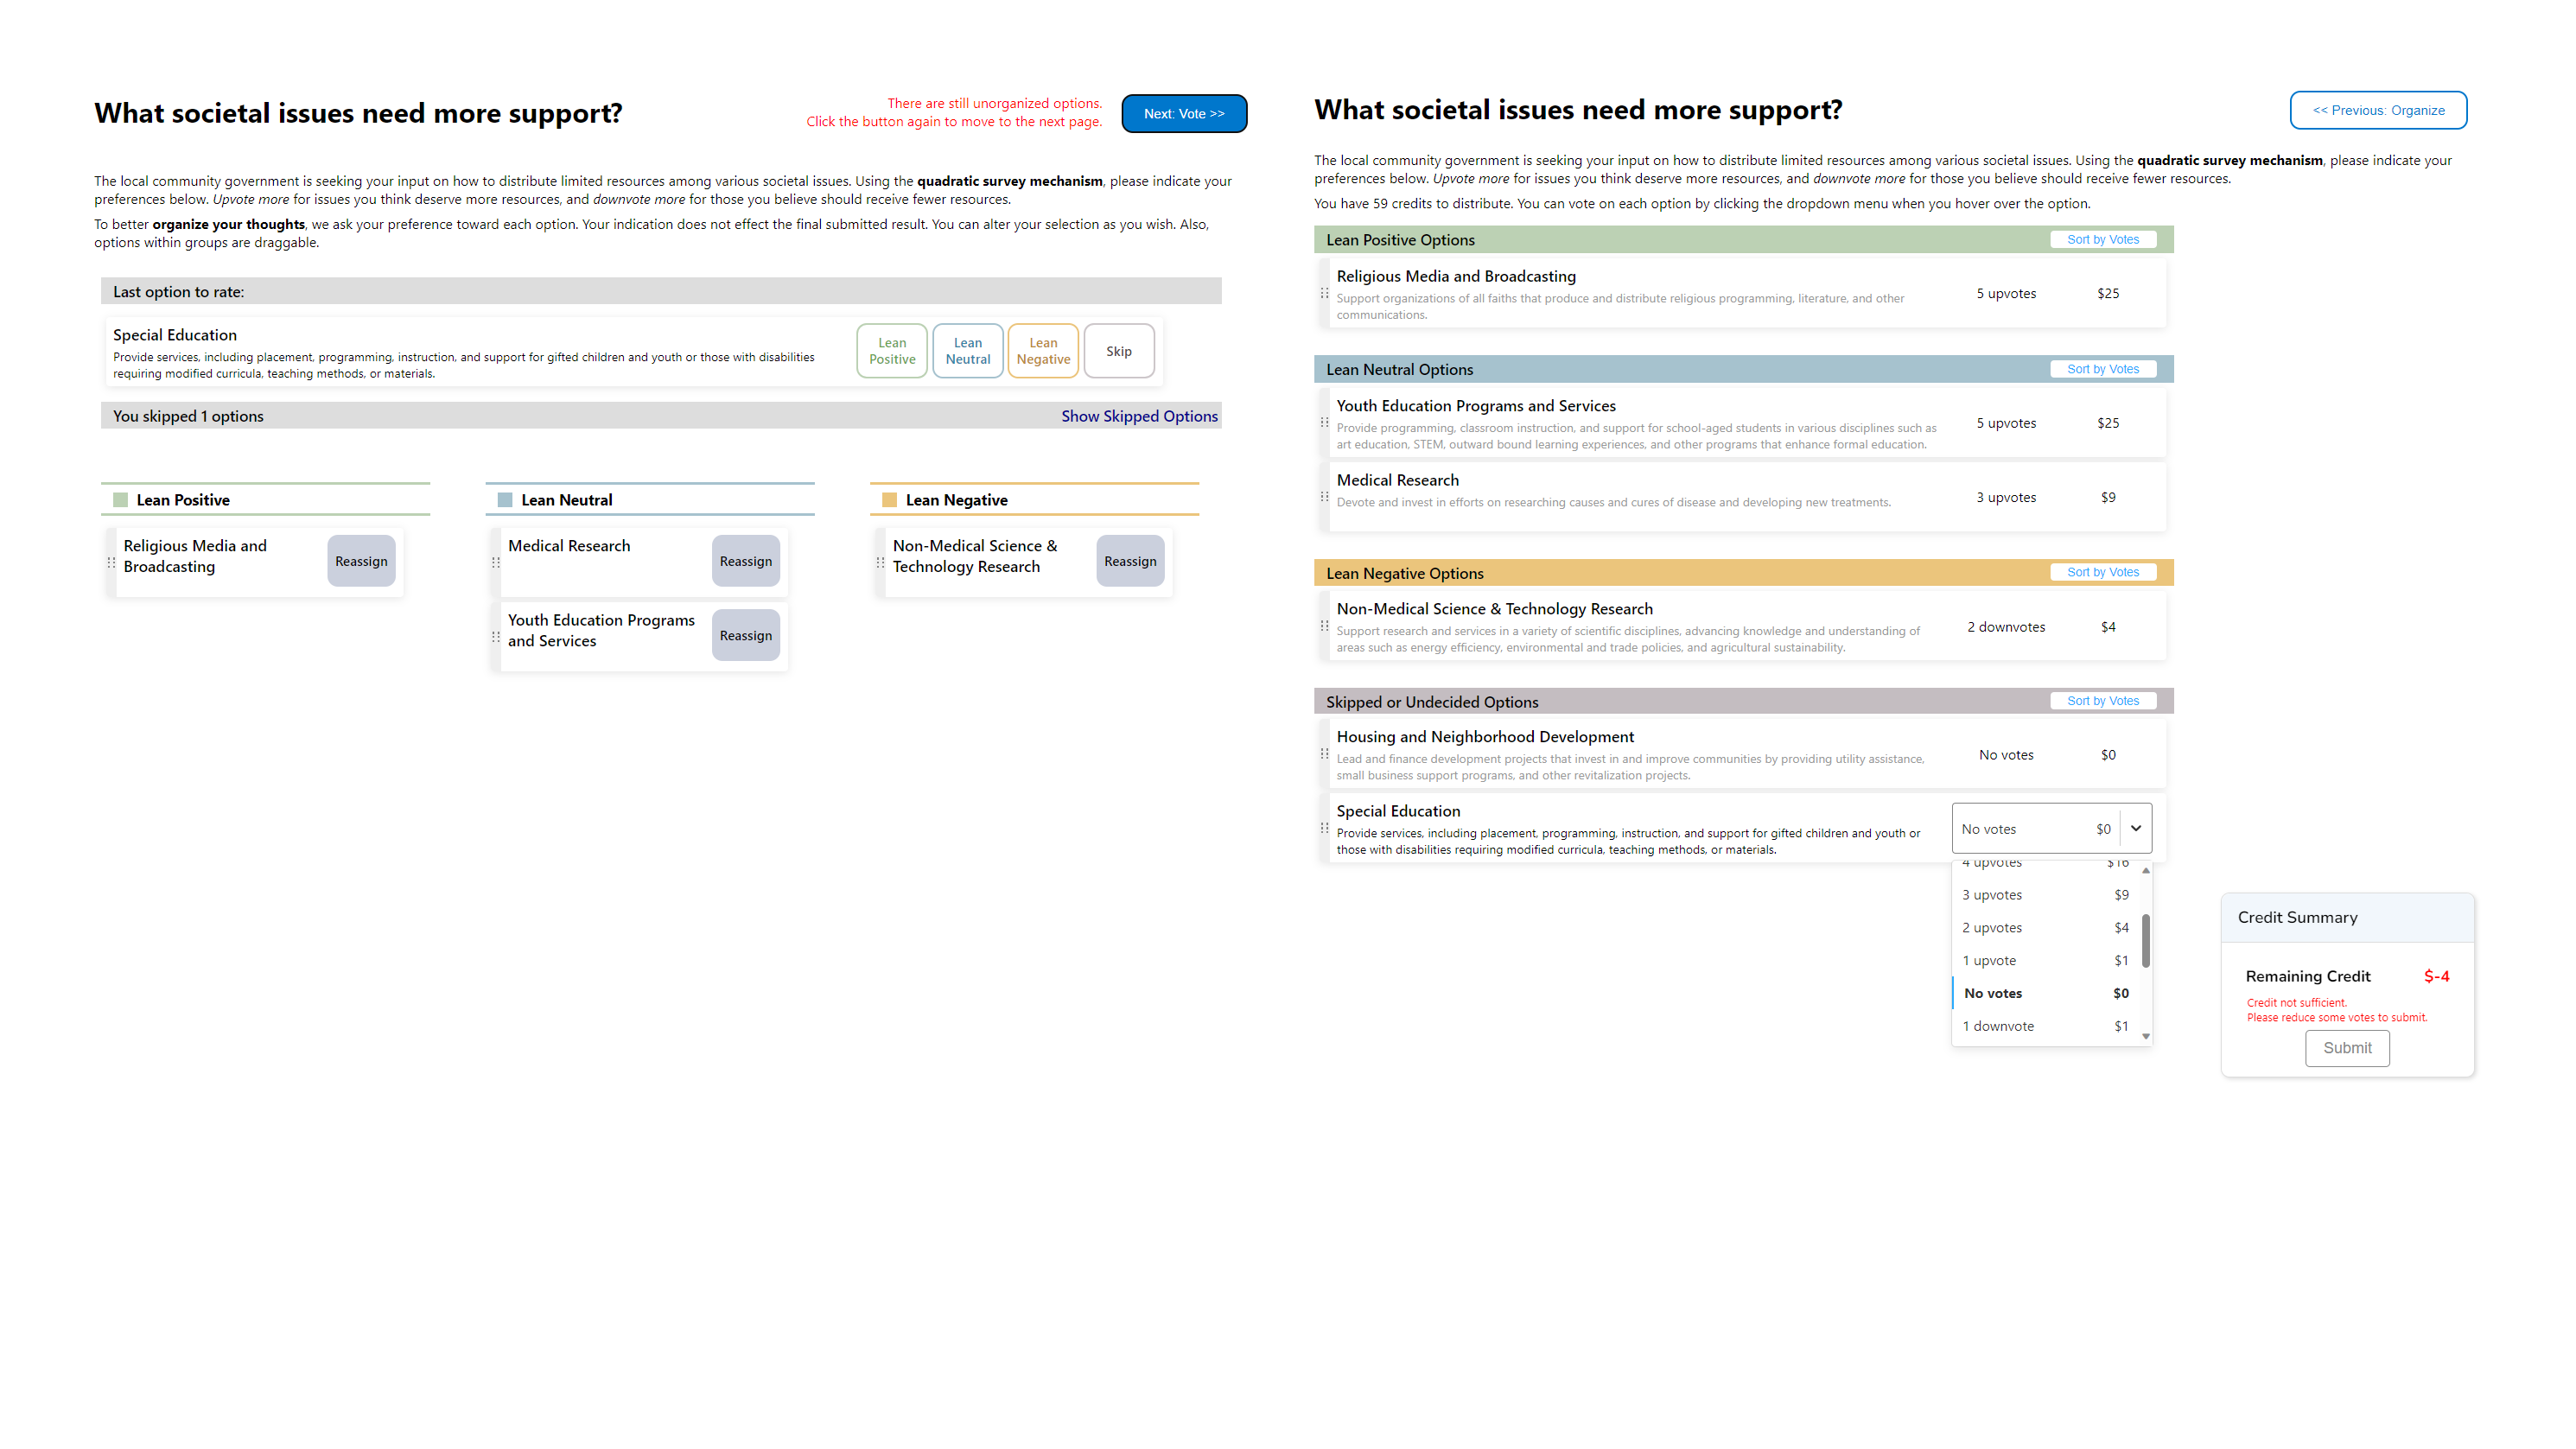
\includegraphics[width=1\textwidth]{content/image/interface.png}
    \caption{The interactive interface}
    \label{fig:interactiveInterface}
\end{figure}

\paragraph{Interactive voting interface}
Given that survey respondents conveyed a rough categorization of options, the voting interface presents the options as they were categorized on the interface, rather than in a randomly ordered manner like the text-based interface. As presented on the right-hand side of Figure~\ref{fig:interactiveInterface}, options are placed in the order of lean positive, lean neutral, lean negative, and skipped or undecided. Undecided options include options that remained in the organization queue. This could happen since survey respondents might have a pre-existing preference or do not want to organize their thoughts. The order within these categories is also preserved. Survey respondents can also choose to go back to the organization interface to focus on updating their choice architecture anytime throughout the survey.

The other difference for the interactive voting interface is that options are draggable for participants to reposition options. Each category also includes a sort-by-vote function to change the position of options within the same `category.' Survey respondents are aware that these additional interface interaction designs will not influence the voting outcome.

These interactions aim to support the positional proximity in information organization. The goal is to partially automate (i.e., automatic positioning of groups) while providing a straightforward mechanism (i.e., drag-and-drop) such that `similar' options and information are placed near each other, allowing participants to process decisions together, echoing research on the proximity compatibility principle~\cite{wickens1995proximity}, specifically spatial proximity~\cite{wickens1990proximity}, and mental compatibility.

While there are various interaction mechanisms to adjust the ordering of options, the notion of drag-and-drop has been explored widely in rank-based surveys. For instance,~\textcite{krosnick2018measurement} demonstrated that replacing drag-and-drop with traditional number-filling rank-based questions improved participants' satisfaction with little trade-off in their time. A similar work embedded drag-and-drop as part of its ranking process~\cite{timbrook2013comparison}. Even though the drag-and-drop interface might lower the stability of the outcome, since we are not trying to capture the position of the options as our final solution, it is worth its trade-off for which survey respondents express a higher satisfactory affordability and ease of use~\cite{rintoulVisualAnimatedResponse}.

Together, these design decisions lead to our belief that a two-step interactive interface with direct interface manipulation can reduce the cognitive load for survey respondents to form preference decisions when completing QS.

\section{Experiment Design}
Based on the design decisions, we developed a QS interface using a React.js frontend and a Next.js backend powered on MongoDB. Both systems are open-sourced~\footnote{link-to-github}.

We recruited participants from a midwestern college town using online ads, digital bulletins, social media posts, physical flyers, and online newsletters. The study's researcher prioritized the non-student population to maximize participant diversity. This study is reviewed and approved by the college Institutional Review Board.

\begin{figure}[h]
    \centering
    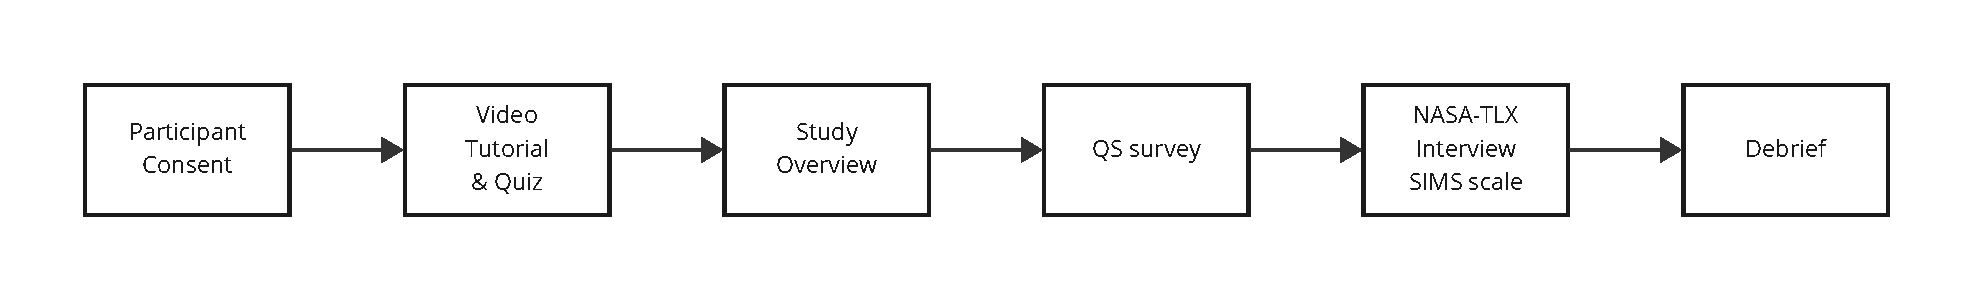
\includegraphics[width=1\textwidth]{content/image/study_flow.pdf}
    \caption{Study protocol}
    \label{fig:studyProtocol}
\end{figure}

Figure~\ref{fig:studyProtocol} shows a visual representation of the study protocol. Study participants are invited to the lab to participate in this study. The reason we made this experiment design decision is to minimize the influence of external factors that could affect the measurement of cognitive load. External factors, more prevalent in remote experiments or those conducted via platforms like MTurk, include potential multitasking or interruptions by others. An in-lab study also allows participants to operate across a consistent device that researchers have full control over. More specifically, the experiment involves participants operating on a 32-inch vertical monitor. This setup assured study participants, despite any condition in the study, can see all options on a QS, minimizing hidden information from an individual's decision-making process.

After consenting to the study, participants are invited to the study and they watch a pre-recorded video explaining the Quadratic mechanism and how QS operates. This video does not include any hints of either interface and how to operate the interface. Participants are then asked to complete a short quiz. The purpose of the quiz is to ensure that all participants fully understand how QS works. Participants are not screened out if they fail the quiz but are asked to rewatch the video or ask the researcher until they are able to select the correct answer. The device that the participant worked on is screen captured throughout the study.

The researcher then primes the participant that the purpose of this study is to assist local community organizers in understanding community members' preferences on a wide variety of societal issues so they can potentially distribute limited resources better. Participants would be randomly placed into one of the four groups:

\begin{itemize}
    \item 6 options with text-based interface
    \item 6 options with iteractive interface
    \item 24 options with text-based interface
    \item 24 options with iteractive interface
\end{itemize}

Participants will begin completing the survey independently, without the researcher's presence. Upon completion, they contact the researcher, who then requests they complete the NASA-TLX to assess cognitive load. This is followed by a short semi-structured interview to gain insights into the participants' experiences. This interview is audio recorded. Finally, participants complete the situational motivation scale (SIMS) to gauge motivation and a demographic survey. The session concludes with a debriefing and a \$15 cash compensation for their participation. The debreifing explains to the participant regarding not disclosing the purpose of the survey is to measure cognitive load and interface design and allows for participants to ask any questions.

The study is designed as a between-subject study for two reasons. First, we aim to minimize the study fatigue that might occur given the complexity of responding to a QS. To complete a QS survey, participants can take up to 20 minutes. Thus, it is difficult to conduct back-to-back experiments that measure cognitive load. We choose not to ask participants to revisit the lab with several days in between, to reduce dropout rates and prevent demotivating participants from attending the in-person experiment, which might occur in a within-subject study design. Second, we aim to reduce the learning effect that is difficult to remove, especially concerning operating the interface and making decisions on the survey. Recall that preferences are constructed, we want to ensure that participants are not influenced by their previous preferences which can influence their perceived cognitive load.

In an ideal world, understanding participants' cognitive load across multiple options would require enumerating all possible numbers of options and eliciting the ``breaking point'' where the participant experiences cognitive overload. Unfortunately, this is not feasible. Iterating through all possible numbers of options is very costly, both in time and resources. Therefore, we refer to prior literature to inform our choice of 6 and 24 options, representing a short and long list of options. To decide the number for the short list, survey methods such as constant sum surveys and Analytic Hierarchy Process (AHP) recommend options fewer than ten and seven, respectively~\cite{moroneyQuestionnaireDesignHow2019, saatyGroupDecisionMaking2013, saatyPrinciplesAnalyticHierarchy1987}. However, we are not aware of any specific works that justify these numbers.~\textcite{saatyPrinciplesAnalyticHierarchy1987} associated this value with both the cognitive processing capacity of $7\pm2$~\cite{millerMagicalNumberSeven1956} and a theoretical proof using the consistency ratio of a pairwise comparison metric~\cite{saaty2003magic}. This informs our decision to contain a pair of dependent variables above and below seven options. We turn to experiments designed to study choice overload. A meta-analysis by~\textcite{chernevChoiceOverloadConceptual2015} surveyed 99 choice overload experiments (N = 7202) and summarized that 6 and 24 are the modal values for short and long lists when testing choice overload. These two values are likely rooted in the original choice overload experiment by~\textcite{iyengarWhenChoiceDemotivating2000}. The value six is often used in experiments to understand the effect of choice provision. The value 24 is the maximum number of ecologically valid jams produced by the jam company in the original study. We decided to follow suit with these two values, satisfying the previous decision to choose two values less than and greater than seven.

Next, we describe the context of the survey that participants completed. Participants were asked to complete a societal issue survey. We follow suit as described by~\textcite{chengCanShowWhat2021}, believing that surveying societal issues is a good topic as it is relevant to every citizen and it is easy to convey that there are limited resources in the public sector to be prioritized across different sectors and areas. Participants across all four groups were presented with options randomly drawn from 26 societal issues. These issues were generated from the categories used by Charity Navigator~\cite{CharityNavigatorAnimals2023}, a non-profit organization that evaluates over 20 thousand charities in the United States. The full list of these societal issues is provided in Appendix B.

Last, we describe the two quantitative measurements taken during the study: cognitive load and motivation. At the time of this study, several methods existed to measure cognitive load, including performance measures, psychophysiological measures, subjective measures, and analytical measures~\cite{gaoMentalWorkloadMeasurement2013}. Given the nature of QS, a task requiring a long period, adopting performance measures like secondary-task measures in our experiment proved challenging due to the difficulty of designing a secondary task. The secondary task must use the same cognitive resources as the primary tasks, and the cognitive resource for completing the survey would vary among participants. Similarly, psychophysiological measures such as pupil size~\cite{palinkoEstimatingCognitiveLoad2010} and ECG~\cite{haapalainenPsychophysiologicalMeasuresAssessing2010} can be highly sensitive to external environments and costly to obtain. Consequently, we relied primarily on subjective measures via self-report surveys and analytical measures like time and clicks collected via the interface. We adopted a paper-based weighted NASA Task Load Index (NASA TLX), a multidimensional scoring procedure using the weighted average of six subscale scores to represent overall workload. Weighted NASA-TLX uses a priori workload definitions from subjects to weight and average subscale ratings, requiring subjects to evaluate each weight's contribution to the workload of a specific task~\cite{hart1988development, hartNasaTaskLoadIndex2006, cain2007review}. This approach reduces between-rater variability, indicating differences in workload definitions among raters within a task and variations in workload sources between tasks~\cite{cain2007review}. Despite criticisms regarding its validity and vulnerability, NASA-TLX is commonly used due to its low cost and ease of administration~\cite{gaoMentalWorkloadMeasurement2013}. It has been tested on various experimental and lab tasks, and workload scores derived from these tests showed significantly less variability among evaluators than one-dimensional workload scores~\cite{rubioEvaluationSubjectiveMental2004}. Thus, we chose NASA-TLX to measure cognitive load in our study.

In addition to NASA-TLX, we administered a situational motivation scale (SIMS) to measure participants' motivation (required citation). We posited that motivation would influence mental demand (required citation). SIMS, chosen for its widespread use, helps understand one's intrinsic motivation, extrinsic motivation, identified regulation, and external regulation, and was originally designed to measure self-determination. Both instruments were administered using pen-and-paper.